\subsection{Installer une distribution}

\begin{tcbenumerate}[3]
    \tcbitem Aller sur la page de téléchargement de \href{https://miktex.org/download}{\bfseries\color{monrose}MikTeX - https://miktex.org/download} et choisir la version \textbf{adaptée à votre système d'exploitation}.\\
    \tcbitem \textbf{Cocher} l'option \textbf{installer les packages à la volée} ( on-the-fly ) pour permettre plus de souplesse dans les premières compilations.\\
    \tcbitem \textbf{Décocher} l'option d'installation pour tous les utilisateurs. Cela rend plus simple l'utilisation de la console MikTeX.
\end{tcbenumerate}

\subsection{Ajouter un localtexmf}

Il s'agit d'un \acc{répertoire} respectant une \acc{structure précise} qui, une fois configuré est automatiquement utilisable par le compilateur \LaTeX\ comme \acc{dossier de packages}.
\begin{MultiColonnes}{2}
    \tcbitem Suivre les étapes suivantes \textbf{une seule fois} :
    \begin{tcbenumerate}
        \tcbitem Coller le dossier \textbf{localtexmf} récupéré sur ma \vocnoindexref{https://github.com/Romain1099/BFCours/tree/7f394e248e9647fe99ff78c01aaf89658ccf6b6d}{page GitHub} \textbf{n'importe ou sur votre machine}. L'essentiel est qu'il reste à cet emplacement. 
        \tcbitem Copier le chemin d'accès de ce dossier. \\
        \tcbitem Ouvrir la \bouton{console MikTeX} et aller au menu \bouton{Settings}.
        \tcbitem Aller dans l'onglet \frquote{Directories}.
        \tcbitem Appuyer sur le bouton \bouton{+} et \textbf{coller} le chemin d'accès au dossier \textbf{localtexmf}.
        \tcbitem Confirmer les changements et quitter la console. 
    \end{tcbenumerate}
    \tcbitem[valign=center] \dirtree{%
        .1 localtexmf/.
        .2 tex/.
        .3 latex/.
        .4 MonPackage/.
        .5 \textcolor{red}{MonPackage.sty}\DTcomment{fichier principal}.
        .5 fichier\_de\_package.sty.
    }
    \begin{center}
        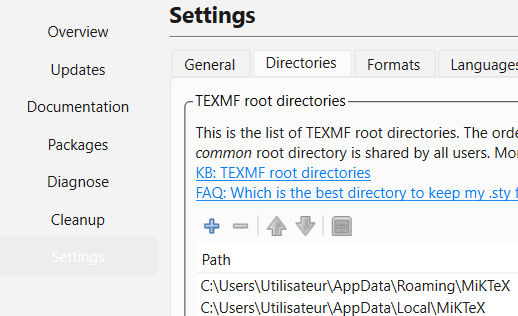
\includegraphics[width=0.75\textwidth]{images/miktex/set_localtexmf_path.png}
    \end{center}
\end{MultiColonnes}

\subsection{Installer VSCode}

Le logiciel VSCode peut être remplacé par un autre IDE s'appuyant sur cette technologie comme \acc{windsurf} ou \acc{cursor}.


\begin{tcbenumerate}[3]
    \tcbitem Aller sur la page de téléchargement de \href{https://code.visualstudio.com/download}{\bfseries\color{monrose}VSCode - https://code.visualstudio.com/download} et choisir la version \textbf{adaptée à votre système d'exploitation}.\\
    \tcbitem Laisser dans un premier temps les paramètres par défaut.
    \tcbitem Il est possible de consulter des \acc{tutoriels} en vidéo pour éditer le \acc{style} de l'IDE. 

    Tout est personnalisable.
\end{tcbenumerate}



\subsection{Installer les extensions VSCode}



\begin{MultiColonnes}{2}
    \tcbitem Puisque VSCode est un outil à \acc{destination des développeurs}, il dispose de nombreuses extensions. 

Il convient d'explorer la bibliothèque d'extension qui prend la forme d'une \acc{marketplace}. 

Par \acc{précaution}, on se limitera à des extensions téléchargées de nombreuses fois et ayant \acc{plusieurs étoiles}. 

    \tcbitem[halign=center] 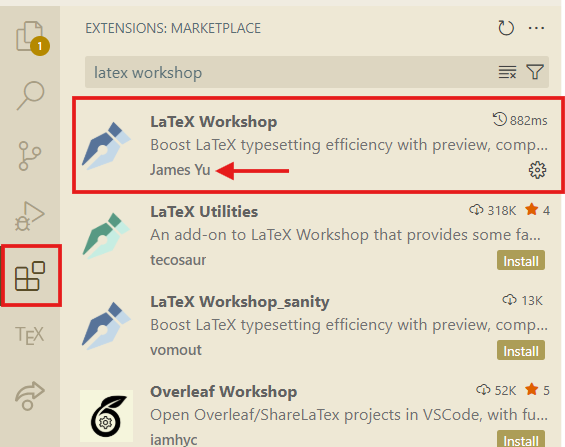
\includegraphics[width=0.75\textwidth]{images/IDE/extension_marketplace.png}
\end{MultiColonnes}


Il y a assez peu d'extensions à télécharger : 

\begin{None}
    \begin{tcbenumerate}[2]
        \tcbitem \acc{LaTeX Workshop}

        Inclut toutes les fonctionnalités de compilation automatique, visualisation de pdf.
        \begin{center}
            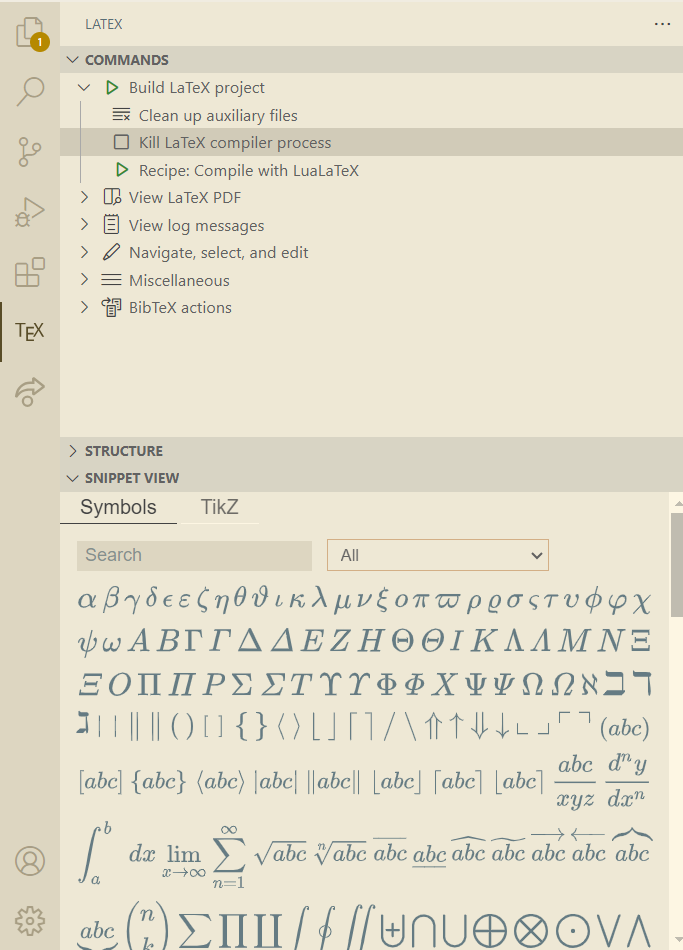
\includegraphics[width=0.9\textwidth]{images/IDE/latex_workshop.png}
        \end{center}

        \tcbitem \acc{git} 

        Pour le suivi et la gestion des modifications. C'est un incontournable surtout lorsqu'on utilise activement des agents IA. 

        \begin{center}
            
\includegraphics[width=8cm]{images/IDE/git_extension_pack.png}
        \end{center}

        \begin{Remarque}[Compilation dans VSCode]

            Il est nécessaire d'\acc{expliquer} à VSCode vos préférences de compilation. 

            Pour cela : 

            \begin{tcbenumerate}[1][1][alph]
                \tcbitem Ouvrir les \acc{settings} de l'extension \acc{LaTeX Workshop}. 

                \bouton{Barre de recherche} $\Longrightarrow$ \bouton{>latex workshop settings} $\Longrightarrow$ \bouton{>settings Sync: Open User Settings(JSON)} 

                \tcbitem Ouvrir le fichier json de settings et \acc{coller} le contenu du fichier ci-après. 

                \tcbitem Désormais, à chaque sauvegarde, le fichier se compile automatiquement et son affichage dans le prévisualisateur pdf est automatiquement actualisé. 
            \end{tcbenumerate}

        \end{Remarque}
        \tcbitem[raster multicolumn=2]  Sur VSCode, il est possible de \acc{partager une session de travail} entre 
        
        \begin{MultiColonnes}{3}
                \tcbitem[raster multicolumn=2] plusieurs participants via l'extension \voc{Live Share}.
                
                Il suffit de lire le \frquote{README} du projet pour se rendre compte de la facilité d'utilisation.
                \tcbitem[halign=center] 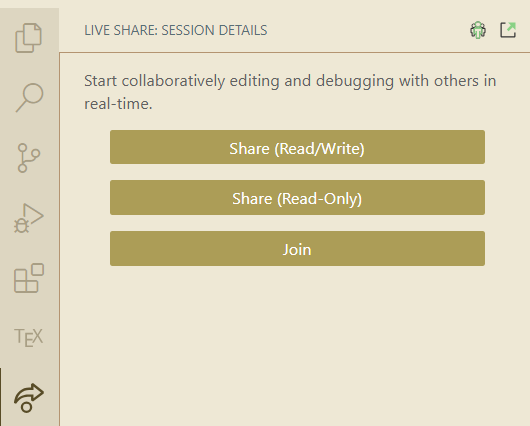
\includegraphics[width=0.55\textwidth]{images/IDE/live_share_snippet.png}
            \end{MultiColonnes}
    \end{tcbenumerate}
\end{None}

\newpage

\begin{Exemple}[Organiser vscode]

    Une fois configuré, votre environnement de travail devrait ressembler à ceci : 

    \begin{center}
        \begin{tikzpicture}
            % Image de base
            \node[anchor=center, inner sep=0] (image) at (0,0) {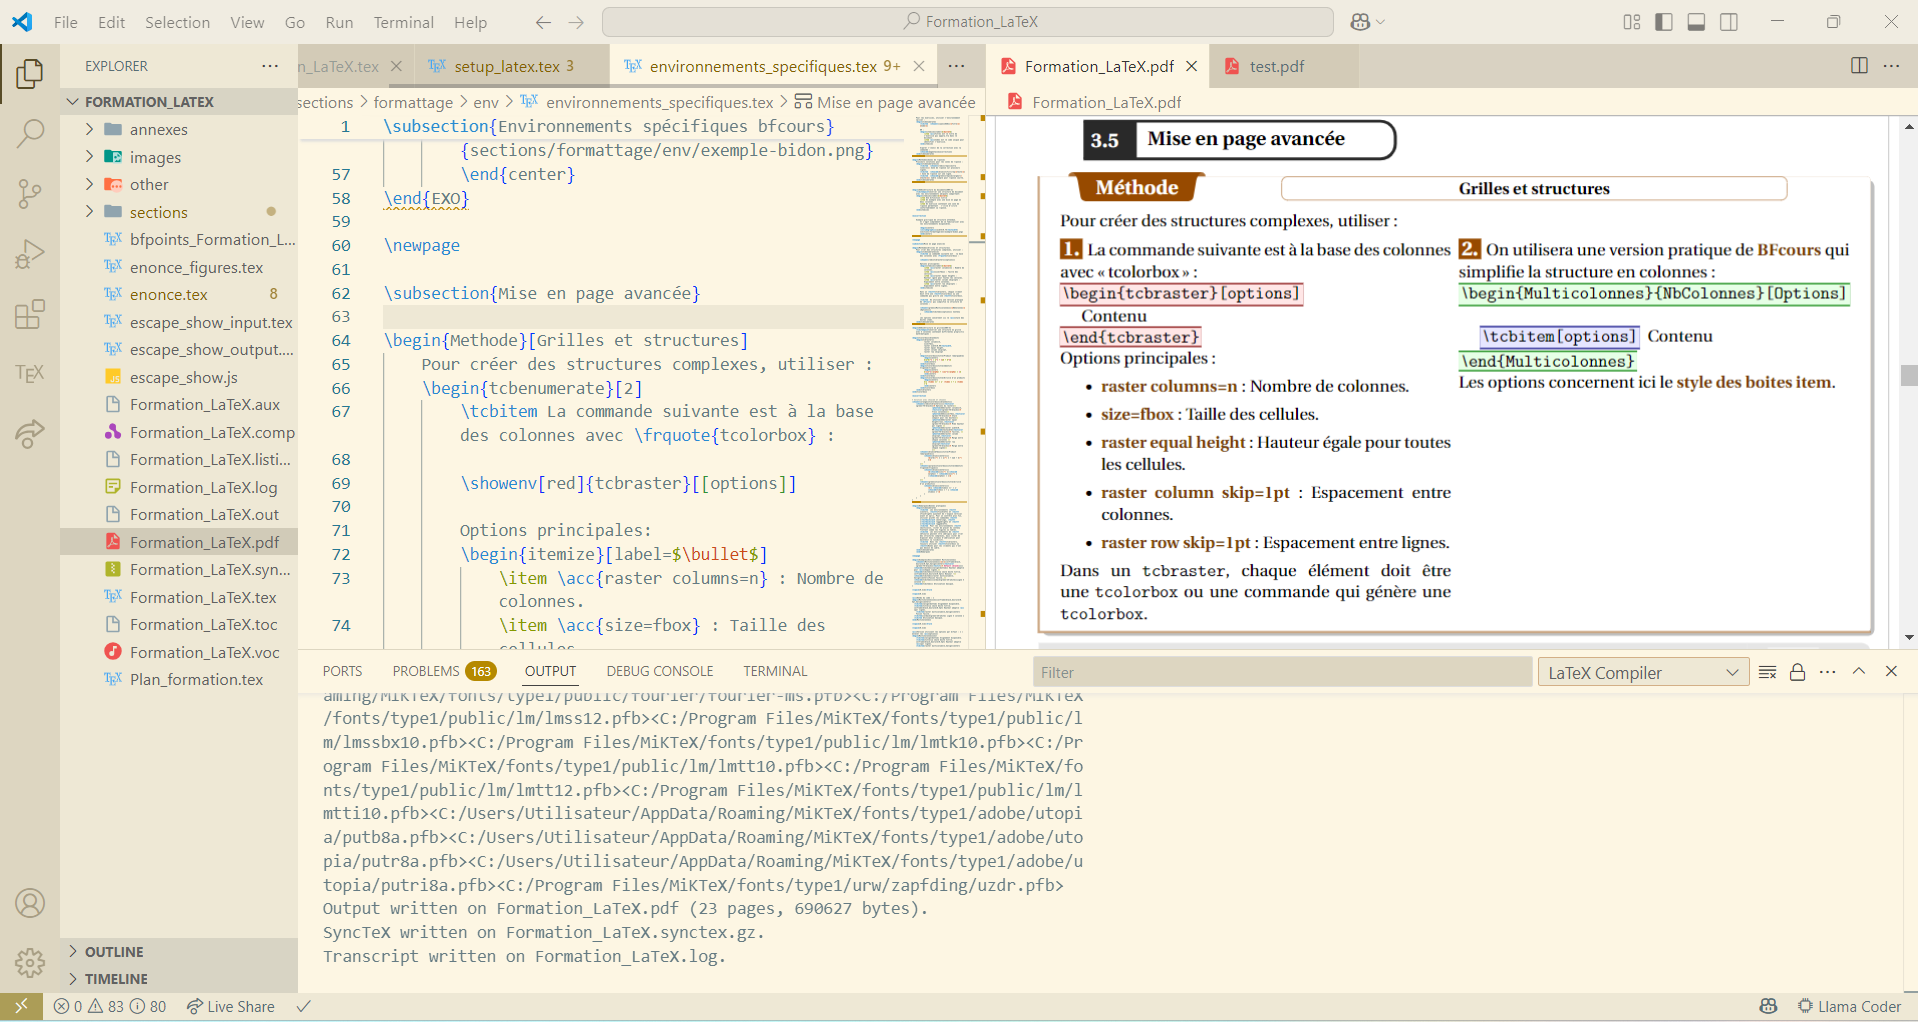
\includegraphics[width=0.8\textwidth]{images/IDE/VSCode_use.png}};
            
            % Obtenir les dimensions de l'image
            \pgfgetlastxy{\maxx}{\maxy}
            
            % Style pour les pastilles
            \tikzset{
                pastille/.style={
                    circle, 
                    fill=red!90!black, 
                    text=white, 
                    font=\bfseries\footnotesize,
                    minimum size=20pt,
                    inner sep=0pt,
                    draw=white,
                    line width=1.5pt
                }
            }
            
            % Placement des pastilles (positions relatives à l'image)
            % 1. Options générales - coin supérieur gauche
            \node[pastille] at (-7, 3.7) {1 $\rightarrow$};
            
            % 2. Barre de recherche - centre haut
            \node[pastille] at (0, 3.8) {2};
            
            % 3. Géométrie voulue pour le terminal - bas
            \node[pastille] at (4.2, 3.7) {3};
            
            % 4. La sidebar - gauche
            \node[pastille] at (-7, 0.5) {4 $ \uparrow $};
            
            % 5. Zone d'exploration - gauche dans la sidebar
            \node[pastille] at (-6, 1.5) {5};
            
            % 6. Onglets - haut du contenu principal
            \node[pastille] at (-2, 3) {6};
            
            % 7. Zone de saisie principale - centre
            \node[pastille] at (-2.5, 0) {7};
            
            % 8. Zone d'affichage secondaire - droite
            \node[pastille] at (3.5, 0) {8};
            
            % 9. Terminal - tout en bas
            \node[pastille] at (0, -2.2) {9};
        \end{tikzpicture}
    \end{center}

    On observe : 
    \begin{tcbenumerate}[2]
        \tcbitem Options générales
        \tcbitem Barre de recherche
        \tcbitem Géométrie voulue pour le terminal
        \tcbitem La \acc{sidebar}
        \tcbitem La zone d'exploration ( fichiers, extensions, recherche sur fichiers multiples )
        \tcbitem Onglets
        \tcbitem Zone de saisie principale
        \tcbitem Zone d'affichage ou de saisie secondaire
        \tcbitem Terminal - permet également d'afficher les logs : 

        \bouton{OUTPUT}$\rightarrow$\bouton{Latex Compiler}
    \end{tcbenumerate}
\end{Exemple}

\newpage

\begin{lstlisting}[language=json]
{
    "terminal.explorerKind": "external",
    "terminal.external.windowsExec": "\"C:\\Windows\\System32\\WindowsPowerShell\\v1.0\\powershell.exe\"",
    "terminal.integrated.shellIntegration.enabled": false,
    "terminal.integrated.env.windows": {
        "PATH": "${env:PATH};C:\\Program Files (x86)\\sox-14-4-2"
    },
    "latex-workshop.latex.tools": [
    {
      "name": "lualatex",
      "command": "lualatex",
      "args": [
        "-synctex=1",
        "-interaction=nonstopmode",
        "-file-line-error",
        "%DOC%"
      ]
    }
  ],
  "latex-workshop.latex.recipes": [
    {
      "name": "Compile with LuaLaTeX",
      "tools": ["lualatex"]
    }
  ],
  "latex-workshop.latex.autoBuild.run": "onSave",
  "editor.wordWrap": "on",
  "editor.cursorBlinking": "expand",
  "editor.cursorSmoothCaretAnimation": "on",
  "workbench.iconTheme": "material-icon-theme",
  "editor.mouseWheelZoom": true,
  "github.copilot.enable": {
    "*": false,
    "plaintext": false,
    "markdown": false,
    "scminput": false,
    "latex": false
  },
}
\end{lstlisting}

\newpage

\begin{EXO}{Le fameux 'Hello world !'}{SET-1}

    \begin{tcbenumerate}
        \tcbitem Ouvrir le fichier \displayFilePath{fichiers\_de\_la\_formation/1.Exercices\_formattage/hello\_world/hello\_world.tex}.
        \tcbitem Appuyer sur \bouton{CTRL+s} ou \bouton{Compiler} pour compiler ce document. 
    \end{tcbenumerate}

    \begin{bfbox}{Structure d'un document latex}
        \showcmd{documentclass}[[a4paper,11pt,fleqn]\{article\}]\mycomment{Définition de la classe du document}\\

        \mycomment{Définition de la géométrie du document}\\
        \showcmd{usepackage}[[left=1cm,right=1cm,top=0.5cm,bottom=2cm]\{geometry\}]\\

        \mycomment{Appel des packages}\\
        \showcmd{usepackage}[[french]\{babel\}] \mycomment{Options spécifiques à la langue française}\\
        \showcmd{usepackage}[\{xcolor\}] \mycomment{Utilisation des couleurs}\\
        \showcmd{usepackage}[\{fourier\}] \mycomment{Police de caractère}\\

        \mycomment{Définition de commandes}\\
        \showcmd[purple]{newcommand}[\{$\backslash$tester\}\{test\}]\\

        \mycomment{Début du document}\\
        \showcmd[red]{begin}[\{document\}] \\

        \phantom{AAA}Hello world !\\

        \phantom{AAA}\showcmd[purple]{tester} \mycomment{\'Ecrira 'test'}\\

        \showcmd[red]{end}[\{document\}]\mycomment{Fin du document}
    \end{bfbox}
\end{EXO}